\section{Konzeption zweier konkreter Lösungen}

Im Folgenden sollen nun zwei konkrete Lösungen zur Erzeugung von Test- bzw. Betriebsumgebungen skizziert werden. Die konkret verwendeten Virtualisierungslösungen werden dabei von der Pixelhouse GmbH vorgegeben.

Zum einen setzt die Pixelhouse GmbH bereits Oracles VirtualBox ein, um eine lokale Entwicklungsumgebung für die Anwendung der Webseite chefkoch.de auf den Laptops der Entwickler vorzuhalten. VirtualBox ist somit bereits auf fast allen Rechnern vorhanden und es existieren grundlegende Kenntnisse und Erfahrungen für dieses Produkt.

Zum anderen wird aktuell von Seiten der Server-Administratoren das Produkt Docker eingeführt, um die Produktivumgebung der Plattform zu betreiben. Diverse Produktiv-Komponenten der Webseite chefkoch.de laufen also bereits innerhalb von Linux-Containern. Die ersten Erfahrungen der Administratoren sind dabei vielversprechend. Es besteht der Wunsch, Probleme zu minimieren, die auftreten, weil Entwicklungs-, Test- und Produktivumgebungen nicht die gleiche Technologie verwenden und sich so grundlegend voneinander unterscheiden.

Nachfolgend soll nun zunächst die aktuelle Produktiv- und die aktuellen Testumgebungen beschrieben werden. Anschließend soll eine Betriebsumgebung definiert werden, die im Rahmen dieser Arbeit die Lösbarkeit der bisherigen Probleme mit Hilfe der Virtualisierungstechnologien zeigen kann. Zudem sollen die eingangs in der Problemstellung angedeuteten Probleme bei der Ausführung von Tests genauer erläutert und durch eine stark vereinfachte Anwendung inklusive entsprechend vereinfachter Tests dargestellt werden. Anschließend kann dann für die beiden Produkte VirtualBox und Docker ein Konzept erarbeitet werden, wie sich diese Umgebung mit Hilfe der entsprechenden Technologie virtualisieren lässt, um damit die zuvor definierte Anwendung und ihre Tests erfolgreich auszuführen.

\subsection{Beschreibung der aktuellen Produktivumgebung}

Die Betriebsumgebung die von der Pixelhouse GmbH in Produktion eingesetzt wird und täglich mehrere Millionen Anfragen von Besuchern der Webseite chefkoch.de beantwortet, besteht aus einer Vielzahl von Komponenten und Diensten. Bis auf die unternehmensweite Groupwarelösung (E-Mails, Kalender, etc.), die bereits als mehrere Dienste in Docker-Containern virtualisert wird, handelt es sich dabei um echte Maschinen, die jeweils auf ihrer eigenen Hardware laufen.

\begin{figure}[!ht]
  \begin{center}
    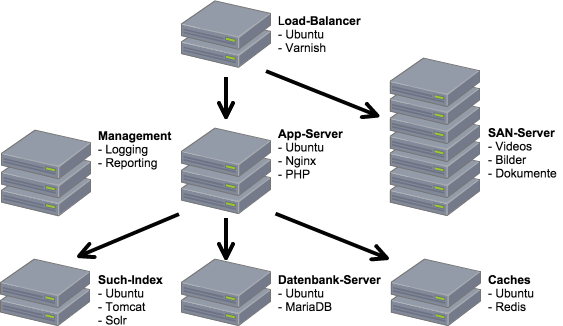
\includegraphics[width=10cm]{bilder/Produktiv-Umgebung.png}
    \caption{Die Produktiv-Umgebung der Webseite chefkoch.de}
  \end{center}
\end{figure}

Im Zentrum der Infrastruktur stehen insgesamt drei Appserver. Bei jedem Appserver handelt es sich dabei um einen Ubuntu-Server, auf dem der Webserver Nginx und der Script-Interpreter PHP ausgeführt wird, um HTTP-Anfragen mit Hilfe statischer oder dynamische Inhalte zu beantworten. Für die langfristige Datenhaltung greifen die PHP-Scripte dabei auf zwei Datenbankserver (Master und Slave) zu, auf denen ebenfalls Ubuntu und der Mysql-Fork MariaDB installiert sind. Für kurzfristige und hochverfügbare Datencaches gibt es zwei Ubuntu-Server (Master und Slave) auf denen der Key-Value-Store Redis läuft. Zudem wird auf weiteren zwei Ubuntu-Servern (Master und Slave) ein Such-Index mit Hilfe der Suchmaschine Solr betrieben, die als Java-Anwendung in einem Tomcat-Application-Server läuft. Binärdateien (Videos, Bilder, Dokumente, etc.) werden auf insgesamt 7 weiteren Servern redundant abgelegt. Damit die Appserver und die SAN-Server von außen unter einheitlichen HTTP-Adressen erreichbar sind und sich die Last gleichmäßig auf die einzelnen Server verteilt, landen sämtliche HTTP-Anfragen per DNS-Round-Robin zunächst bei einem von zwei Ubuntu-Servern, auf denen Varnish als Load-Balancer installiert ist. Diese nehmen die Anfragen entgegen und verteilen sie an die dahinter liegenden Server. Varnish ist zudem ein effizienter HTTP-Cache, der in der Lage ist, die von den App- oder SAN-Servern zurückgelieferten Antworten zu cachen und bei erneuter Anfrage selbst auszuliefern. Zu guter Letzt gibt es noch drei weitere Server, auf denen Software für die Administration und das Reporting läuft.

\subsection{Beschreibung der aktuellen Testumgebungen}

Die aktuellen Testumgebungen der Pixelhouse GmbH besitzen einen extrem reduzierten Aufbau. Die Testumgebungen werden alle auf ein und derselben Hardware-Maschine installiert. Fast alle Komponenten der zuvor beschriebenen Produktiv-Umgebung werden dabei von den einzelnen Testumgebungen gemeinsam verwendet. Beispielsweise nutzen alle Testumgebungen den gleichen Varnish für Load-Balancing und Caching. Dieser reicht die HTTP-Anfragen an den selben Nginx-Web-Server und PHP-Interpreter weiter und cached die Antworten bei Bedarf gleichermaßen. Als Backend-Dienste werden dieselbe MariaDB-Datenbank, derselbe Redis-Cache und derselbe Solr-Such-Index verwendet. Die Binärdateien werden ebenfalls auf demselben Host von allen Testumgebungen gemeinsam verwendet. Einziger Unterschied zwischen den einzelnen Testumgebungen ist, dass aufgrund einer speziellen Konfiguration im Nginx-Webserver je nach aufgerufener URL vom PHP-Interpreter andere PHP-Scripte geladen werden und somit jeweils eine andere Version der PHP-Anwendung getestet werden kann.

\begin{figure}[!ht]
  \begin{center}
    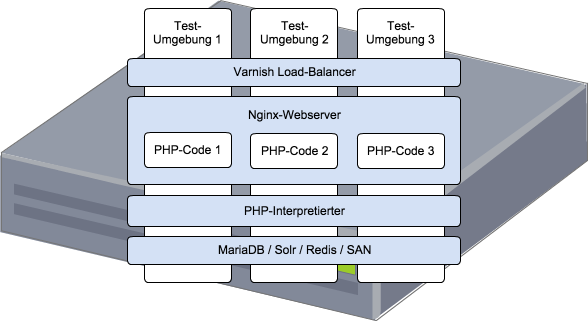
\includegraphics[width=10cm]{bilder/Aktuelle-Testumgebung.png}
    \caption{Die aktuelle Test-Umgebung}
  \end{center}
\end{figure}

Die aktuelle Testumgebung bringt Probleme in Bezug auf die Testbarkeit der Anwendung mit sich. Da alle Testumgebungen zum Beispiel die gleichen Backend-Dienste verwenden, ist es mitunter nicht möglich, die für den Test notwendigen Testdaten zu erzeugen, ohne damit Einfluss auf andere Testumgebungen zu nehmen. Ein weiteres Problem ist, dass nur Änderungen am PHP-Code selbst testbar sind. Will man zum Beispiel eine Änderung am HTTP-Caching im Varnish testen, kann man diese nur in allen Testumgebungen gleichermaßen vornehmen.

\subsection{Definition einer verifizierbaren Testumgebung}

Um nun eine zwar möglichst leicht zu implementierende, für die Darstellung der Lösbarkeit dieser Probleme aber hinreichende Umgebung zu definieren, werden folgende Änderungen vorgenommen:
Zunächst wird die Anzahl gleicher Komponenten auf jeweils eins reduziert. Außerdem werden die Caches und der Such-Index ausgeblendet, da sie genau wie die Datenbankserver aus den Appserver heraus als Backend-Dienst abgefragt werden und lediglich eine andere Technologie beziehungsweise einen anderen Schwerpunkt der Datenhaltung widerspiegeln (Kurzfristigkeit und Durchsuchbarkeit). Zuletzt ignorieren wir im Rahmen dieser Arbeit die SAN- und Management-Server.

Die von uns definierte Umgebung besteht somit lediglich aus einem Varnish-Load-Balancer, einem Nginx-Appserver, der den Script-Interpreter PHP ausführt und einen Maria-DB-Server, der aus PHP heraus als Backend-Dienst abgefragt werden kann.

Eine solche Umgebung könnte nun mit Hilfe von Virtualisierung mehrmals parallel auf einer physischen Maschine gestartet werden.

\begin{figure}[!ht]
  \begin{center}
    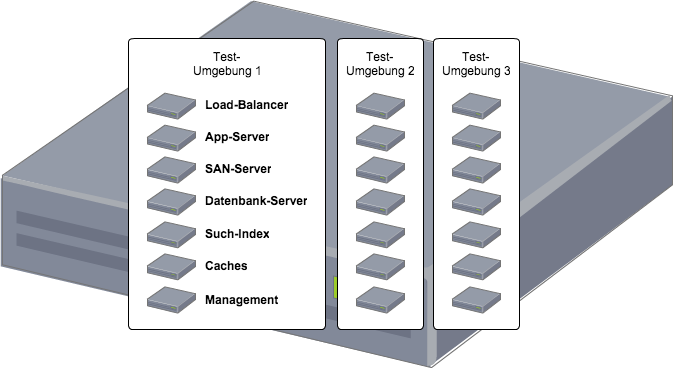
\includegraphics[width=10cm]{bilder/Untersuchungs-Umgebung.png}
    \caption{Für die Untersuchung definierte Umgebung}
  \end{center}
\end{figure}

\subsection{Definition von Anwendungs- und Testfällen}

Für die Verifizierung der jeweiligen Testumgebungen ist es notwendig, eine andere PHP-Anwendung als die echte Anwendung der Webseite chefkoch.de zu verwenden. Zum einen ist die echte PHP-Anwendung auf dieser reduzierten Testumgebung nicht lauffähig. Zum anderen hat sie im Laufe der Jahre eine Komplexität erreicht, die es schwer macht, einen einfachen Anwendungsfall zu finden, der dennoch die Notwendigkeit von isolierten Testumgebungen aufzeigt.

Es ist deshalb von Vorteil, im Rahmen dieser Arbeit neue PHP-Scripte mit einzelnen Anwendungsfällen zu definieren, die die zuvor angedeuteten Probleme beim Ausführen der Tests, die auf eine mangelnde Isolation einzelner Test-Umgebungen zurückzuführen sind, einfach provozieren. Passend dazu lassen sich dann ebenso einfache Testfälle definieren, die zeigen, ob die neue Testumgebungen mit Hilfe der Virtualisierungstechnologien die eingangs erläuterten Probleme einfach lösen.

\subsubsection{Isolierte Testdaten in der Datenbank}

Wir denken uns einen einfachen Anwendungsfall aus, der Daten derart in die Datenbank schreibt, dass es Einfluss auf andere Testumgebungen haben würde, wenn sich mehrere Testumgebungen die gleiche Datenbank teilen. Dazu reicht es zum Beispiel aus, einen einfachen Zähler zu implementieren. Dieser Zähler legt zunächst, falls noch nicht vorhanden, eine neue Tabelle an, die eine Integer-Spalte enthält und fügt einen Datensatz mit dem Wert 1 ein. Falls die Tabelle schon existiert, erhöht er den Wert um eins. Der aktuelle Wert wird anschließend ausgegeben. Dieser Anwendungsfall sollte also beim ersten Aufruf eine 1 ausgeben und bei jedem weiteren Aufruf einen um eins erhöhten Wert (2, 3, 4, 5...).

Zum Test der Testdaten-Isolierung muss man nun lediglich zwei Testumgebungen anlegen und sicherstellen, dass beide Umgebungen unabhängig voneinander zählen.

\subsubsection{Konfigurationsänderung im HTTP-Cache}

Um eine Änderung am HTTP-Caching zu testen, brauchen wir zunächst ein einfaches PHP-Script, das zum einen die aktuelle Uhrzeit ausgibt und zum anderen einen HTTP-Cache-Header mitsendet, der HTTP-Caches dazu veranlasst, die HTTP-Antwort für 10 Sekunden zu cachen.
Es ist nun per Varnish-Konfiguration möglich, diese HTTP-Header für bestimmte URLs zu berücksichtigen oder eben nicht.

Damit sollte es möglich sein, eine Testumgebung zu starten, die beim Aufruf des PHP-Scriptes immer die aktuelle Uhrzeit anzeigt. Gleichzeitig muss es möglich sein, eine weitere Testumgebung zu starten, in der das gleiche HTTP-Cache nur alle 10 Sekunden die aktuelle Uhrzeit anzeigt.

\subsubsection{Behat als Testframework}

Natürlich ist es möglich, die zuvor beschriebenen Tests wie auch echte Tests zur Webseite chefkoch.de händisch durchzuführen. Vorgabe der Pixelhouse GmbH ist es aber, die Durchführung von Tests zu automatisieren. Die Pixelhouse GmbH hat sich bei der Wahl eines entsprechenden Testframeworks für das Tool Behat entschieden. Dies liegt zum einen daran, dass Behat selbst auch in der Programmiersprache PHP geschrieben ist und somit die notwendige Kompetenz zur Implementierung solcher Testfälle bereits vorhanden ist. Behat ist außerdem ein sogenanntes Behaviour-Driven-Development Tool. Dies meint, dass die eigentliche Definition der Testfälle in Form von menschenlesbarem Text erfolgt, der das gewünschte Verhalten der Anwendung beschreibt.

\begin{figure}[!ht]
  \begin{center}
    \begin{gherkincode}
Feature: Counter
  In order to know how often I visited the counter page
  the counter has to increase with every visit

  Scenario:
    Given I open "/counter.php"
    Then I should see "1"
    When I reload the page
    Then I should see "2"

    \end{gherkincode}
    \caption{Beispiel-Feature für den Zähler}
  \end{center}
\end{figure}

Solche Feature oder auch User Story genannten Beschreibungen werden von der Pixelhouse GmbH bereits im Rahmen ihrer Entwicklungsmethode Scrum verwendet, um die Kommunikation zwischen Produktmanagement und Entwicklern zu formalisieren.

\subsection{VirtualBox}

Um die zuvor definierte Testumgebung mit VirtualBox zu virtualisieren, ist es zunächst sinnvoll, fertige virtuelle Maschinen zu erzeugen, die sich bei Bedarf direkt mit VirtualBox starten lassen. Ein Werkzeug zur Erzeugung solcher Maschinenabbilder ist Packer.

Es wäre außerdem von Vorteil, das Starten der einzelnen Maschinen nicht selbstständig steuern zu müssen. Ein Werkzeug, mit dem man mehrere virtuelle Maschinen zu einer Gesamtumgebung auf Basis von VirtualBox orchestrieren kann, ist Vagrant.

Im Folgenden wird nun die Funktionsweise der beiden Werkzeuge Packer und Vagrant genauer beschrieben.

\subsubsection{Erzeugung der einzelnen Maschinen mit Packer}

Packer ist ein Werkzeug zur Erzeugung eindeutiger Maschinenabbilder für verschiedene Plattformen auf Basis einer einfachen Konfiguration. Packer kennt dabei vor allem drei wichtige Konzepte: Builder, Provisioner und Post-Processor. Diese werden mit Hilfe der Konfigurations-Datei packer.json definiert:

\begin{figure}[!ht]
  \begin{center}
    \begin{jsoncode}
{
    "description": "Varnish-Image",
    "builders": [
        {
            "type": "virtualbox-ovf",
            "source_path": "ubuntu-14.04.ovf"
        }
    ],
    "provisioners": [
        {
            "type": "shell",
            "script": "/pfad/zum/script-das-varnish-installiert.sh"
        }
    ],
    "post-processors": [
        {
            "type": "vagrant",
            "output": "varnish.box"
        }
    ]
}
    \end{jsoncode}
    \caption{Einfaches Beispiel einer packer.json}
  \end{center}
\end{figure}

Ein Builder beschreibt eine bestimmte Technologie, mit deren Hilfe das virtuelle Maschinen-Abbild erzeugt wird. Neben verschiedenen anderen Technologien beinhaltet Packer auch Builder zur Erzeugung von virtuellen Maschinen mit VirtualBox. Grundsätzlich gibt es dabei zwei Möglichkeiten: Zum einen kann man einen Builder vom Typ "`virtualbox-iso"' verwenden. Mit diesem wird eine leere virtuelle Maschine erzeugt und anschließend mit Hilfe eines Installationsmedium im ISO-Format ein Betriebssystem installiert. Zum anderen kann man einen Builder vom Typ "`virtualbox-ovf"' verwenden. Das Format OVF ist ein generisches Format zum Import und Export von virtuellen Maschinen. Mit diesem Builder kann man also mit Hilfe von Packer ein Maschinen-Abbild auf Basis eines anderen Maschinen-Abbildes erzeugen. So kann man zum Beispiel eine fertig installierte Linux-Distribution als Ausgangspunkt zur Installation weiterer Anwendungsprogramme verwenden. Für die von uns definierte Testumgebung wollen wir die einzelnen virtuellen Maschinen auf Basis einer fertigen Installation von Ubuntu 14.04 Server erzeugen.

Um nun weitere Software auf der mit dem Builder erzeugten virtuellen Maschine zu installieren, kommt ein sogenannter Provisioner zum Einsatz. Ein Provisioner ist für Packer eine Technologie, mit der es einfach möglich ist, solche Installationsvorgänge zu konfigurieren. Dabei gibt es sehr umfangreiche Ansätze wie die Werkzeuge Puppet oder Chef, die sehr mächtige Konfigurationssprachen bieten, um verschiedenste Installations- und Konfigurationsschritte in einem Betriebssystem vorzunehmen. Eine andere, eher einfache Variante wäre aber zum Beispiel der Provisioner vom Typ "`Shell Script"', bei dem eben lediglich ein Shell Script innerhalb der virtuellen Maschine ausgeführt wird, um weitere Einstellungen oder Installationen vorzunehmen. Dieser sehr einfache Ansatz ist für die einzelnen Maschinen unsere beispielhaften Testumgebung ausreichend.

Zu guter Letzt kennt Packer nun noch das Konzept des Post-Prozessors. Ein Post-Prozessor meint dabei eine bestimmte Art und Weise, mit der das fertige Maschinen-Abbild exportiert und für die Verwendung mit anderen Tools vorbereitet wird. So gibt es eben einen Post-Prozessor vom Typ "`Vagrant"', der es ermöglicht, das fertige Maschinen-Abbild direkt mit Vagrant innerhalb einer Testumgebung zu starten. Damit sollte es möglich sein, die einzelnen fertigen virtuellen Maschinen unserer beispielhaften Testumgebung so abzulegen, dass wir sie sofort als Gesamtumgebung starten können.

\subsubsection{Umgebungssteuerung mit Vagrant}

Vagrant bietet eine einfach zu konfigurierende, reproduzierbare und portierbare Betriebsumgebung auf Basis etablierter Virtualisierungs-Technologien und einen einfachen Ansatz zu deren Verwaltung.

\begin{figure}[!ht]
  \begin{center}
    \begin{rubycode}
Vagrant.configure("2") do |config|
  config.vm.define "varnish" do |varnish|
    varnish.vm.box = "varnish"
    varnish.vm.box_url = "file:///varnish.box"
  end

  config.vm.define "mariadb" do |mariadb|
    mariadb.vm.box = "mariadb"
    mariadb.vm.box_url = "file:///mariadb.box"
  end

  # ...
end
    \end{rubycode}
    \caption{Einfaches Beispiel einer Vagrantfile}
  \end{center}
\end{figure}

Dazu legt man zunächst eine Konfigurationsdatei namens Vagrantfile an, in der man seine Umgebung definiert. Vagrant bietet dabei die Möglichkeit eine oder mehrere virtuelle Maschinen auf Basis von verschiedenen Virtualisierungstechnologien zu starten. So bietet es eben auch die Möglichkeit, virtuelle Maschinen mit Hilfe von VirtualBox zu starten, die mit Packer vorbereitet wurden. Es bietet weiterhin einfache Konfigurationsparameter, die zum Beispiel die Netzwerkkommunikation zwischen den virtuellen Maschinen und dem Host-Betriebssystem und auch untereinander ermöglichen. Auch einzelne Parameter wie Anzahl der virtuellen Prozessoren und die Menge des zur Verfügung gestellten Arbeitsspeicher lassen sich hier noch nachträglich definieren. Es ist auch möglich, Ordner zwischen dem Host-Betriebssystem und den virtuellen Maschinen zu teilen, um so zum Beispiel während der Entwicklung mit einer IDE auf dem Host-Betriebssystem Code zu bearbeiten, der direkt in den virtuellen Maschinen ausgeführt wird.

Ist die Konfigurationsdatei fertig, so lässt sich die entsprechende Umgebung mit einem einfach Kommandozeilen-Befehl starten: "`vagrant up"'. Vagrant lädt und startet dann alle in der Konfigurationsdatei angegebenen Maschinen und setzt die gewünschten Konfigurationen für Netzwerkkommunikation, Hardware-Parameter und gemeinsame Ordner um.

Anschließend lässt sich die innerhalb der Umgebung laufende Anwendung zum Beispiel mit einem Browser des Host-Betriebssystems oder eben mit dem Testtool Behat ansteuern.

\subsection{Docker}

Auch bei der Verwendung von Docker zur Virtualisierung der Testumgebung mit Hilfe von OS-Containern stellt sich zunächst die Frage, wie man die einzelnen Container erzeugt. Im Gegensatz zu VirtualBox ist dazu keine weitere Software notwendig, da Docker bereits selbst die Möglichkeit zur Erzeugung solcher Images mit sich bringt. Es ist dazu lediglich notwendig, eine einfach Definitionsdatei, eine sogenannte Dockerfile, zu schreiben.

Die Orchestrierung der einzelnen Container zu einer Gesamtumgebung soll auch Teil von Docker selbst werden. Bislang wird ein entsprechendes Werkzeug aber noch als getrenntes Projekt namens Fig entwickelt.

Sowohl auf die Verwendung der Dockerfiles als auch auf die Verwendung von Fig wird im Folgenden näher eingegangen.

\subsubsection{Images mit Dockerfiles bauen}

Docker bietet eine einfache, integrierte Möglichkeit, neue Maschinen-Abbilder zu erzeugen. Wie im Grundlagen-Kapitel beschrieben, werden diese Maschinen-Abbilder mit Hilfe eines Union-Filesystems gestartet. Einzelne Abbilder lassen sich so durch das Hinzufügen eines weiteren, überlagernden Dateisystems zu neuen Abbildern erweitern. Die Definitions-Datei eines Docker-Images, Dockerfile genannt, startet deshalb immer mit der Angabe des zugrundeliegenden Images. Anschließend lassen sich einfach Kommandozeilen-Befehle definieren, die in der laufenden Maschine ausgeführt werden. Führen diese Befehle zu Änderungen am Dateisystem, so werden diese Änderungen eben in einer neuen Dateisysteme-Ebene festgehalten, die Teil des fertigen Abbildes wird. Genauso einfach lassen sich auch Dateien in die Maschine kopieren, die auf dem Host-System liegen. Schließlich lässt sich auch ein Befehl konfigurieren, der standardmäßig ausgeführt wird, wenn man das Image später als Container startet.

\begin{figure}[!ht]
  \begin{center}
    \begin{dockercode}
FROM ubuntu:14.04
RUN apt-get install -y varnish
ADD /pfad/zur/varnish-config.vcl /etc/varnish/default.vcl
CMD ["varnishd"]
    \end{dockercode}
    \caption{Einfaches Beispiel einer Dockerfile}
  \end{center}
\end{figure}

Ein Image lässt sich dann einfach mit dem Befehl "`docker build -t varnish"' erzeugen. Anschließend lässt sich das Image mit dem Befehl "`docker run varnish"' als Container ausführen. Es ist sogar möglich, das fertige Image mit dem einfachen Befehl "`docker push varnish"' in einem Web-Verzeichnis, der sogenannten docker-registry unter https://registry.hub.docker.com/, zu veröffentlichen. Streng genommen müsste der Name hierbei dann aber der Namenskonvention "`benutzername-bei-docker/varnish"' folgen. So ist es jedem möglich, dieses Image oder auch andere Images des Verzeichnisses als Basis für ein weiteres Image zu verwenden oder auch einfach nur als Container auszuführen.

\subsubsection{Steuerung der Umgebung mit Fig}

Um nun die mit Docker erzeugten Images zu einer Gesamtumgebung zu orchestrieren, bietet sich das Tool Fig an. Dafür muss zunächst eine Konfigurationsdatei namens fig.yml definiert werden, in der die einzelnen Maschinen der Umgebung und weitere Einstellungen wie zum Beispiel zur Netzwerkkommunikation zwischen den Maschinen konfiguriert werden.

\begin{figure}[!ht]
  \begin{center}
    \begin{yamlcode}
varnish:
  image: benutzername-bei-docker/varnish
  ports:
   - "80"

mariadb:
  image: benutzername-bei-docker/mariadb
  ports:
   - "3306"

# ...
    \end{yamlcode}
    \caption{Einfaches Beispiel einer fig.yml}
  \end{center}
\end{figure}

Anschließend lässt sich die Umgebung mit dem einfachen Befehl "`fig up"' starten.
